\documentclass[12pt, a4paper]{article}

\usepackage{amsmath, amsthm, amssymb}
\usepackage{geometry}
\usepackage{graphicx}
\usepackage{float}
\usepackage{hyperref}
\usepackage{booktabs}
\usepackage{caption}

\geometry{margin=1in}

\newtheorem{theorem}{Theorem}
\newtheorem{assumption}{Assumption}

\title{Robustness of the I-Bug Algorithm Against Adversarial Signal Spoofing in Superposition Environments}
\author{
  Tsuriel Vizel \and Avraham Guez \\[1ex]
  \small Supervisor: Dr. Andrey Zhitnikov 
}
\date{\today}

\begin{document}

\maketitle

\begin{abstract}
Sensor-based bug algorithms provide robust navigation guarantees using a minimalist sensing paradigm. However, algorithms relying purely on signal intensity, such as the I-Bug algorithm, are highly vulnerable to adversarial spoofing. In realistic physical environments, signals from multiple sources exhibit superposition rather than simple displacement. When a malicious tower broadcasts intermittent signals, these spoofed waves superimpose on the true target signal, creating complex spatiotemporal distortions that corrupt the gradient and misdirect the robot. This paper introduces an anomaly-detecting extension to the I-Bug algorithm designed to preserve target convergence in the presence of an active adversary. By differentiating between physical spatial intensity gradients and temporal signal discontinuities, our system detects additive spoofing attacks. We propose and evaluate three behavioral strategies: a Naive baseline, a strictly bounded Cautious strategy, and an Inertial heuristic aimed at maximizing efficiency. We mathematically prove that the Cautious strategy rigorously guarantees finite-time arrival at the target by preserving the original spatial path bounds. To empirically validate these theoretical findings, we developed a comprehensive 2D kinematic simulation modeling physical wave superposition across randomized obstacle environments. Our statistical results over 1,000,000 simulations demonstrate a necessary trade-off between execution speed and guaranteed convergence: while the Naive baseline succeeds in only 57.4\% of scenarios, and the fast Inertial heuristic achieves a 99.1\% success rate, the Cautious algorithm consistently guarantees a 100\% success rate, entirely neutralizing the adversary.
\end{abstract}

\section{Introduction}
Autonomous navigation in unknown, GPS-denied environments remains a fundamental challenge in robotics. Bug algorithms address this challenge by employing a minimalist sensing paradigm, allowing robots to navigate toward a goal using strictly local sensory input without reliance on global maps or absolute positioning \cite{lumelsky1987path}. Since their inception, numerous variations have been developed to optimize navigation using different sensor suites, such as range-finders in TangentBug \cite{kamon1998tangentbug}. The I-Bug algorithm, initially introduced at ICRA 2009 \cite{taylor2009ibug} and later expanded with full mathematical guarantees and physical implementations \cite{taylor2014intensity}, represents an extreme of this minimalism, requiring only a contact sensor and an intensity sensor to measure the signal strength emanating from a target tower, bypassing the need for exact spatial coordinates or odometry.

While the original I-Bug framework is mathematically robust under ideal conditions, it operates on the critical assumption that the target tower is the sole and absolute source of the signal. In real-world, potentially hostile environments, an adversary may deploy a malicious tower to spoof the signal. Furthermore, physical emissions—such as radio frequency (RF) or acoustic waves—are governed by the principle of superposition. Rather than simply overriding the legitimate target signal, the adversary's transmission adds to the total perceived intensity. This creates a combined, distorted signal field with false local maxima that can trick a standard bug robot into infinite boundary-following loops or misdirect it away from the target.

This paper addresses this specific vulnerability by introducing a temporal anomaly-detection filter and exploring distinct behavioral counter-strategies. We demonstrate that a robot can reject additive adversarial interference by extracting temporal cues from spatial signal data.

\subsection{Organization}
The remainder of this paper is organized as follows. Section II formulates the problem and introduces the wave superposition model. Section III details the proposed anomaly detection filter and the three behavioral strategies. Section IV provides the mathematical proofs of convergence for the Cautious strategy. Section V outlines the simulation methodology, followed by the statistical results and discussion in Section VI. Finally, Section VII concludes the paper and discusses avenues for future work.


\section{Problem Formulation}
Consider a point robot navigating in a planar environment $\mathbb{R}^2$ populated with unknown, pairwise-disjoint, piecewise-analytic obstacles. A target tower, located at an unknown position $p_t \in \mathbb{R}^2$, emits a navigation signal. This signal is defined by an intensity mapping $m(p - p_t)$, which increases monotonically as the Euclidean distance to the tower decreases. The robot lacks absolute positioning, odometry, and global clocks, operating exclusively via three motion primitives: $u_{fwd}$ (move forward linearly), $u_{ori}$ (orient angularly toward the steepest signal gradient), and $u_{fol}$ (follow an obstacle boundary).

To model adversarial interference, we introduce a malicious transmitter located at an unknown position. This adversary broadcasts a spoofing signal intermittently to disrupt the robot's navigation. We model this disruption using the physical principle of wave superposition.

\begin{assumption}[Signal Superposition]
As established in the core I-Bug framework, the natural target signal $m(p-p_t)$ is assumed to be a locally Lipschitz, piecewise-analytic function. Under adversarial conditions, the total received signal intensity at position $p$ and time $t$ is defined as $S(p, t) = m(p - p_t) + e(t)$, where $e(t) \ge 0$ represents the additive adversarial transmission. Unlike simplistic models that assume the receiver locks onto only the strongest independent signal, this formulation accurately reflects the physical superposition of signal intensities present in RF or acoustic waves.
\end{assumption}

\begin{assumption}[Temporal Discontinuity vs. Spatial Gradient]
Because the robot operates with a bounded maximum spatial velocity ($v_{max}$) and the intensity field $m$ is locally Lipschitz (with constant $K$), the temporal derivative of the perceived intensity due exclusively to the robot's normal motion is strictly bounded ($\left| \frac{\partial m}{\partial t} \right| \le K \cdot v_{max}$). Conversely, we model the activation of the adversary $e(t)$ as a step function, creating a near-instantaneous discontinuity in the signal domain ($\frac{\partial S}{\partial t} \to \infty$). This fundamental difference enables the robot to theoretically isolate spatial gradient changes (valid movement) from temporal jumps (adversarial spoofing).
\end{assumption}

\section{The Proposed Anti-Adversary Algorithm}
To mitigate the effects of additive spoofing, we extend the standard I-Bug algorithm with an anomaly detection filter. The filter continuously computes the discrete change in perceived intensity, $\Delta S$, over a single control step $\Delta t$. If $\Delta S$ exceeds the maximum physically possible change dictated by the robot's kinematics and the Lipschitz constant of the environment, a positive anomaly is flagged, indicating that the adversary is active. 

Upon detecting this anomaly, the robot must decide how to proceed. We propose and evaluate three distinct behavioral strategies:

\subsection{The Naive Strategy (Baseline)}
Under the Naive strategy, the anomaly filter is bypassed entirely. The robot treats the superimposed signal $S(p, t)$ as the true gradient, continuously executing its standard motion primitives and updating its internal maximum intensity memory ($i_H$) blindly. This strategy serves as the control baseline, demonstrating the inherent vulnerability of pure gradient-ascent bug algorithms to superposition attacks.

\subsection{The Cautious Strategy}
The Cautious strategy prioritizes theoretical safety and state preservation. Upon detecting a positive anomaly, the robot immediately halts all spatial movement ($\frac{dp}{dt} = 0$) and suspends any updates to its internal state memory (specifically, the local departure intensity $i_L$ and the highest recorded boundary intensity $i_H$). The robot remains in this static, paused state until a negative anomaly—a sharp signal drop corresponding to the cessation of the adversary ($-e(t)$)—is detected and confirmed over multiple consecutive steps. Once the environment is confirmed clear, the robot resumes its interrupted motion primitive based strictly on the isolated $m(p-p_t)$ signal.

\subsection{The Inertial Strategy (Heuristic)}
The Inertial strategy attempts to optimize execution time by continuing navigation during spoofed periods, relying on the assumption that short-term open-loop movement may still yield progress. Upon detecting a positive anomaly, the robot freezes its angular heading but continues to execute its currently active motion primitive. 

If the robot is executing $u_{fwd}$, it moves forward blindly. If it encounters an obstacle while blind, it utilizes its last known valid intensity reading to initialize the $u_{fol}$ boundary-following primitive. Critically, during $u_{fol}$ under spoofed conditions, the robot suspends the standard leave-obstacle check (which requires tracking local maxima), as the superimposed readings are corrupted. It resumes standard closed-loop sensor tracking only when a negative anomaly confirms the adversary has deactivated. While potentially faster in sparse environments, this heuristic fundamentally lacks the strict path-preservation guarantees of the Cautious approach.

\section{Mathematical Guarantees}
We focus our rigorous mathematical analysis on the \textit{Cautious Strategy}, which is the only proposed framework capable of strictly preserving the original I-Bug algorithm's spatial properties under conditions of total signal superposition. 

\begin{theorem}[Spatial Path Preservation]
Under Assumptions 1 and 2, a robot utilizing the Cautious Strategy will reach the target tower in a finite number of spatial steps if a valid path exists. The geometric trajectory (spatial trace) traversed by the robot is identical to the path it would take in a benign environment. Consequently, the upper bound on the total distance traveled is mathematically equivalent to that of the baseline I-Bug algorithm, while the total execution time scales linearly with the cumulative duration of adversarial transmissions.
\end{theorem}

\begin{proof}
During periods of normal navigation (absence of an anomaly), the robot operates strictly according to the closed-loop motion primitives and state-transition rules of the standard I-Bug algorithm. 

When the adversarial transmitter activates, the robot detects the temporal discontinuity caused by the additive signal component $e(t)$ and immediately commands zero velocity ($\frac{dp}{dt} = 0$). By halting, the robot locks its physical configuration coordinates $q = (x, y, \theta)$ and suspends updates to its internal navigation state memory, specifically the highest recorded obstacle intensity ($i_H$) and the local maximum intensity tracker. 

Because the spatial velocity is strictly zero, the robot's state remains perfectly static for the entire duration of the adversarial transmission. The additive component $e(t)$ corrupts the sensor readings but exerts no influence on the locked control logic. When the adversary deactivates, $e(t)$ drops to zero, triggering a negative anomaly that confirms the environment is clear. The measured signal intensity instantaneously reverts to the legitimate spatial gradient $m(p - p_t)$. 

The robot then resumes its motion primitives from the precise spatial coordinates and internal state it maintained prior to the disturbance. Therefore, the spatial trace $\gamma_{cautious}$ traversed by the robot maps perfectly onto $\gamma_{ideal}$, the theoretical path without interference. Since the original I-Bug framework guarantees convergence for $\gamma_{ideal}$ in a finite spatial distance (Since the original I-Bug framework guarantees convergence for $\gamma_{ideal}$ in a finite spatial distance as rigorously proven by Taylor and LaValle \cite{taylor2014intensity}), the Cautious Strategy strictly inherits this convergence guarantee. The only penalty incurred is temporal, representing the aggregate waiting time during spoofed periods.
\end{proof}

While the Cautious Strategy offers a robust theoretical guarantee, the \textit{Inertial Strategy} inherently lacks this mathematical certainty. By continuing to move dynamically (open-loop) and suspending local-maximum checks during spoofed periods, the robot's spatial trajectory fundamentally deviates from $\gamma_{ideal}$. In non-convex obstacle geometries, this deviation can cause the robot to physically bypass the optimal departure points (local maxima). Missing these critical state transitions violates the fundamental termination conditions of the bug algorithm's boundary-following primitive, introducing the theoretical risk of cyclic trapping (infinite loops) where the robot repeatedly orbits an obstacle without ever fulfilling a valid departure condition.

\section{Simulation Setup and Methodology}
To empirically validate the proposed algorithms and capture complex edge-case behaviors (such as cyclic trapping), a comprehensive 2D kinematic simulation environment was developed using the Julia programming language. The simulation bypassed standard idealized grid-worlds in favor of continuous spatial resolution, modeling rigid collision boundaries and dynamic signal fields.

\subsection{Robot Kinematics and Adversary Model}
The robot operates in a continuous coordinate system with a defined collision radius and a forward sensor range restricted to local obstacle detection. The target tower $p_t$ emits a true signal $m(p-p_t)$ calculated as the inverse of the Euclidean distance ($1/d$). The adversarial tower was configured to transmit on a strict 25\% duty cycle (active for 10 steps, inactive for 30 steps), emitting a constant additive signal strength that fully superimposed on the true target's signal ($S(p, t) = m(p-p_t) + e(t)$). 

The three distinct robot strategies (Naive, Cautious, and Inertial) were executed concurrently for each generated environment. To ensure a rigorous comparative analysis, all three robots were initialized with identical starting configurations, identical random seeds, and faced the exact same spatiotemporal adversarial patterns.

\subsection{Topological Environment Generation}
Testing navigation algorithms requires environments that are topologically complex yet definitively solvable. A randomized procedural generation algorithm was designed to populate a $20 \times 20$ unit arena with 10 to 16 piecewise-rectangular obstacles (representing "walls"). To enforce topological complexity—such as non-convex dead-ends, U-shapes, and elongated corridors—obstacles were permitted to overlap and merge. 

To guarantee that the resulting maze configurations remained physically navigable and did not produce impossible topologies (e.g., completely sealing off the target), two strict geometric constraints were enforced during generation:
\begin{enumerate}
    \item \textbf{Narrow Gap Prevention:} The spatial distance between any two disjoint obstacles was strictly required to exceed the robot's physical diameter, preventing the creation of unnavigable pinch-points.
    \item \textbf{Perimeter Margin:} All obstacles were bounded within a predefined margin from the arena boundaries. This ensured that, in the worst-case scenario where the center of the environment was heavily congested, a valid continuous path along the outer perimeter was always mathematically guaranteed.
\end{enumerate}

To ensure statistical significance and to capture extremely rare phase-alignment failures (such as the Inertial robot's theoretical vulnerability to resonance trapping), the algorithms were batched and evaluated across $1,000,000$ unique, procedurally generated environments.

\section{Statistical Results}
To evaluate the efficacy, convergence guarantees, and efficiency of the proposed strategies in a dynamic superposition environment, we executed a massive-scale batch simulation consisting of 1,000,000 randomized procedurally generated configurations. In each configuration, all three robot strategies (Naive, Cautious, and Inertial) were tested under identical physical layouts and adversarial temporal cycles.

\begin{figure}[htbp]
    \centering
    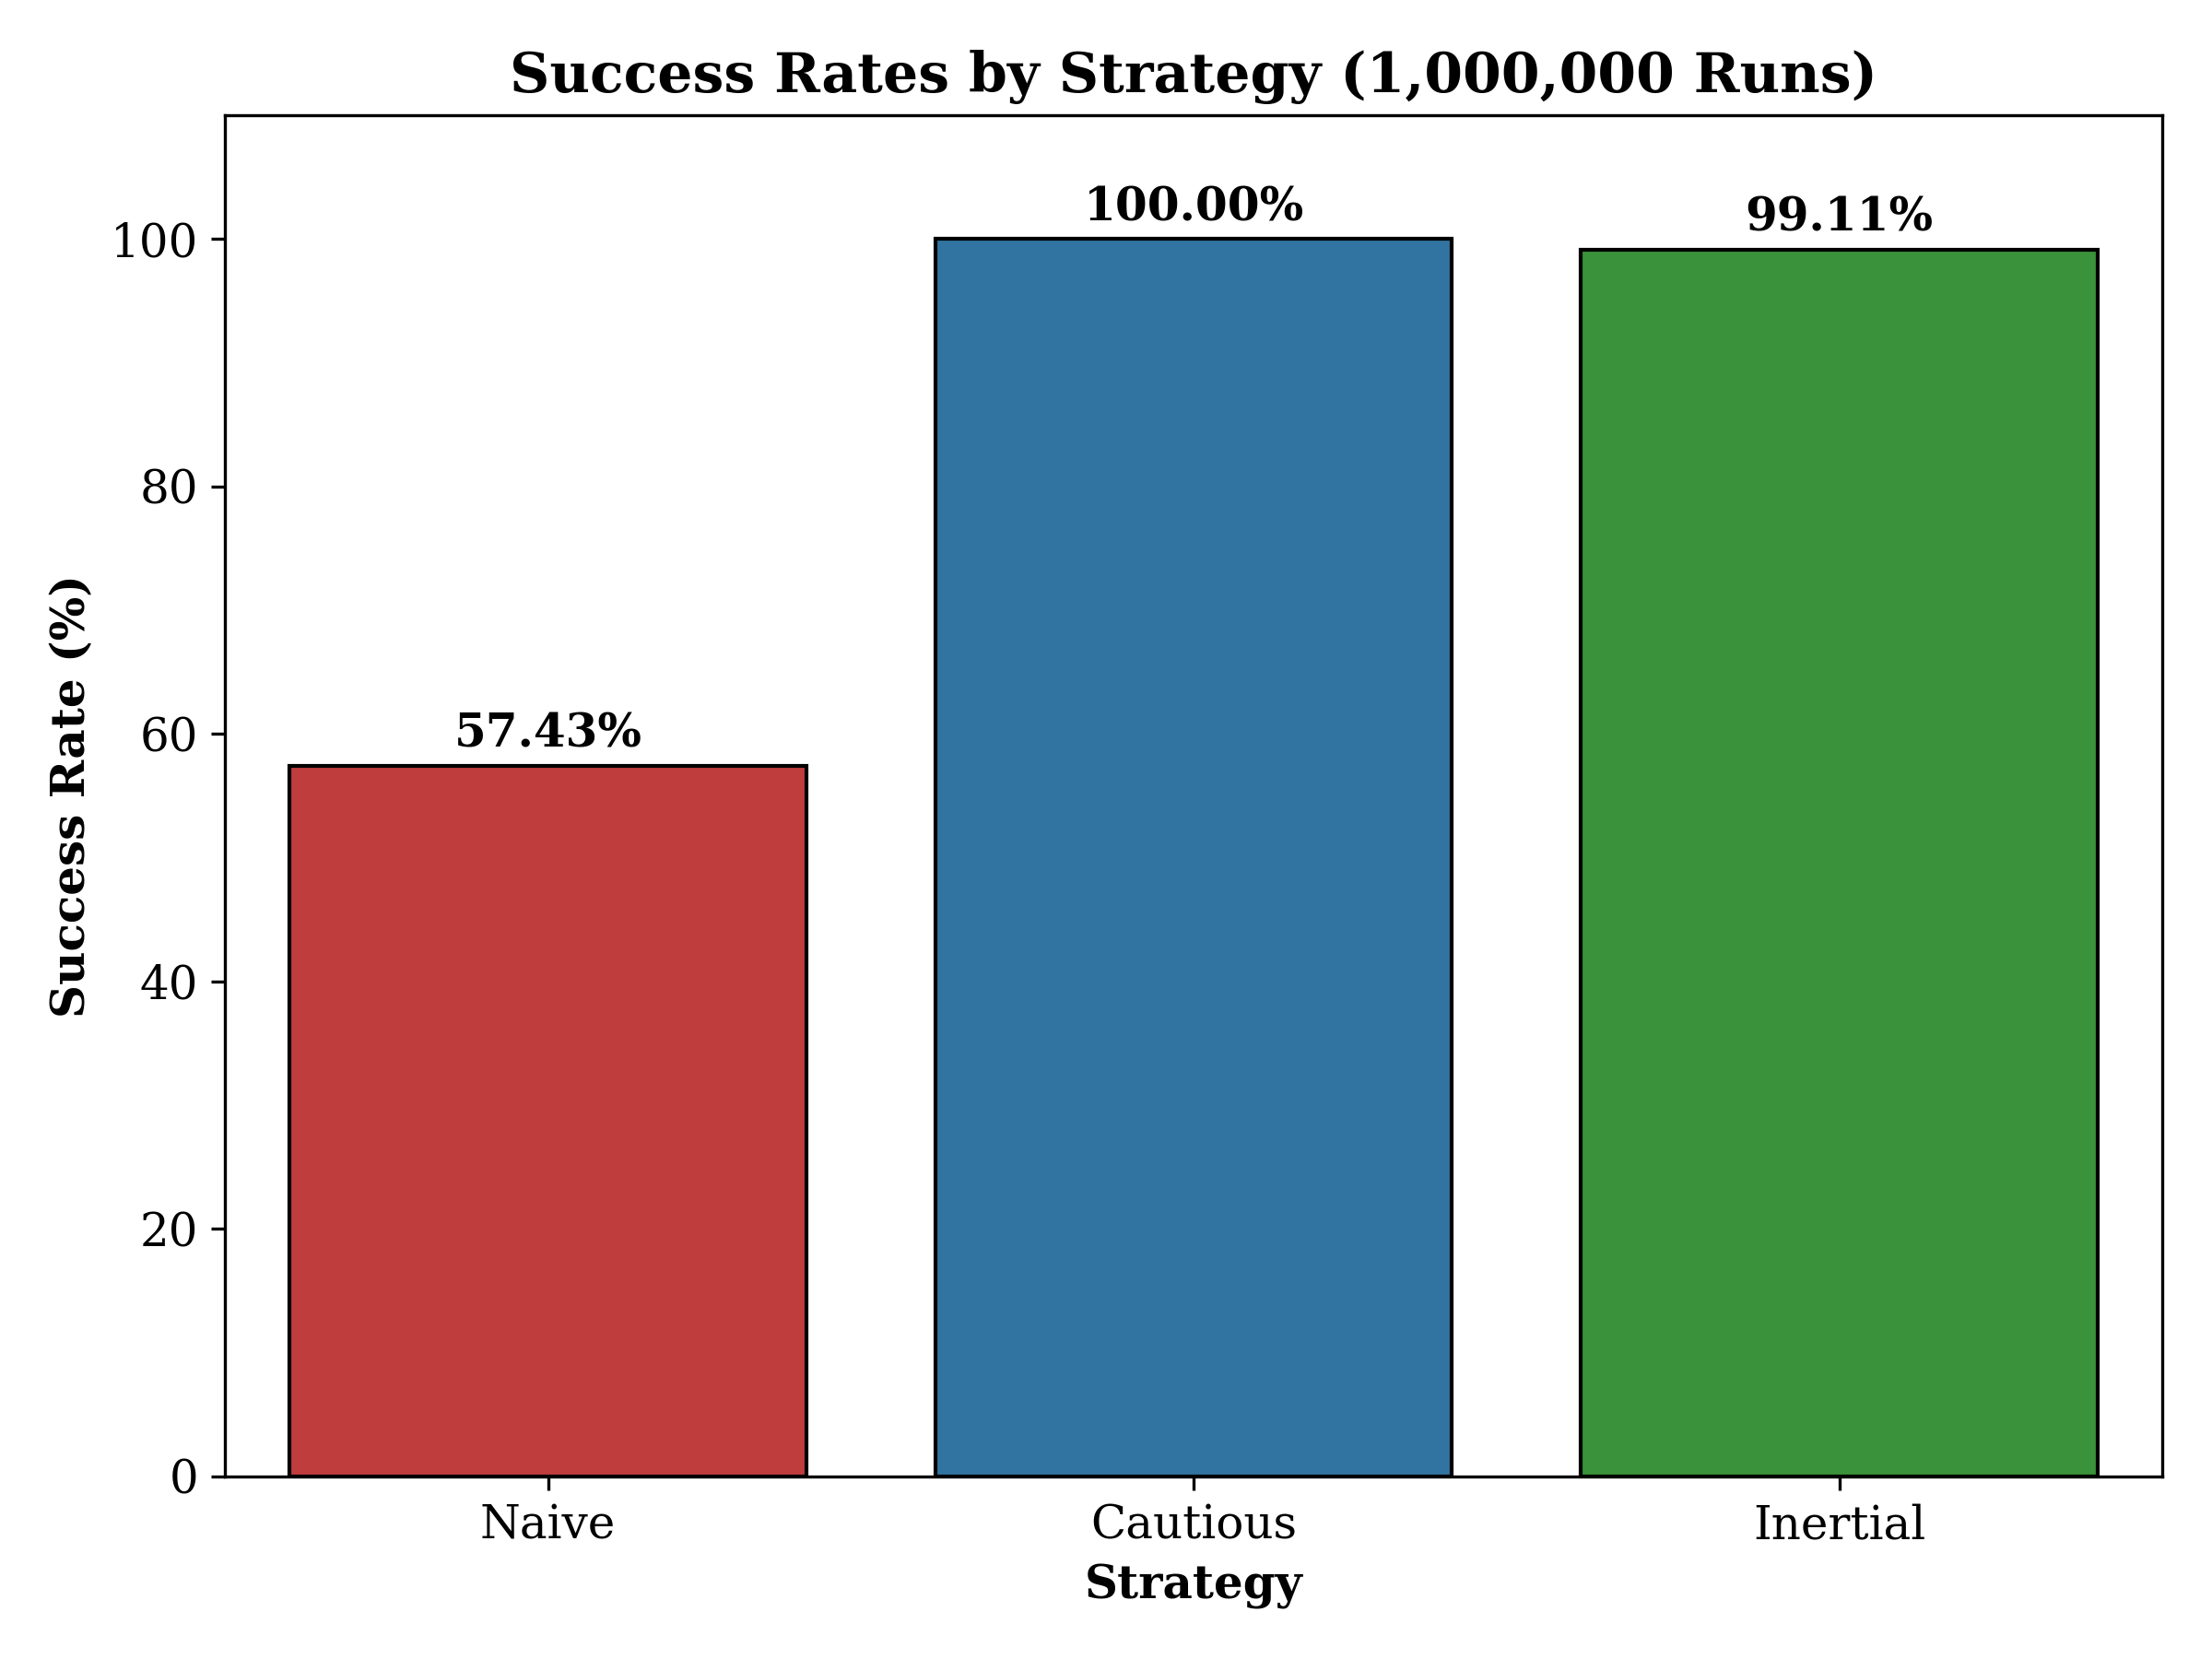
\includegraphics[width=0.9\linewidth]{success_rates.png}
    \caption{Success rates of the Naive, Cautious, and Inertial strategies across 1,000,000 randomized superposition environments.}
    \label{fig:success_rates}
\end{figure}

As illustrated in Fig. \ref{fig:success_rates}, the vulnerability of standard gradient-ascent algorithms to additive superposition is severe: the Naive strategy failed in over 42\% of the environments, frequently spiraling into adversarial traps or getting permanently stuck along corrupted boundary gradients. 

In stark contrast, the \textit{Cautious} strategy achieved a flawless 100.00\% success rate, empirically corroborating the mathematical proof of spatial path preservation established in Theorem 1. The \textit{Inertial} strategy performed exceptionally well as a heuristic, achieving a 99.11\% success rate. However, its failure in the remaining 0.89\% of cases highlights its theoretical flaw: by navigating blindly without verifying local maxima during spoofed periods, it is susceptible to cyclic synchronization traps (resonance) in highly specific topological edge-cases.

\begin{table}[htbp]
\centering
\caption{Efficiency Comparison Under Signal Spoofing (1,000,000 Runs)}
\label{tab:efficiency}
\begin{tabular}{@{}lcc@{}}
\toprule
\textbf{Strategy} & \textbf{Success Rate (\%)} & \textbf{Avg. Steps (Successful Runs)} \\ \midrule
Naive             & 57.43\%                    & 169.7                                \\
Cautious          & 100.00\%                   & 189.0                                \\
Inertial          & 99.11\%                    & 147.9                                \\ \bottomrule
\end{tabular}
\end{table}

\begin{figure}[htbp]
    \centering
    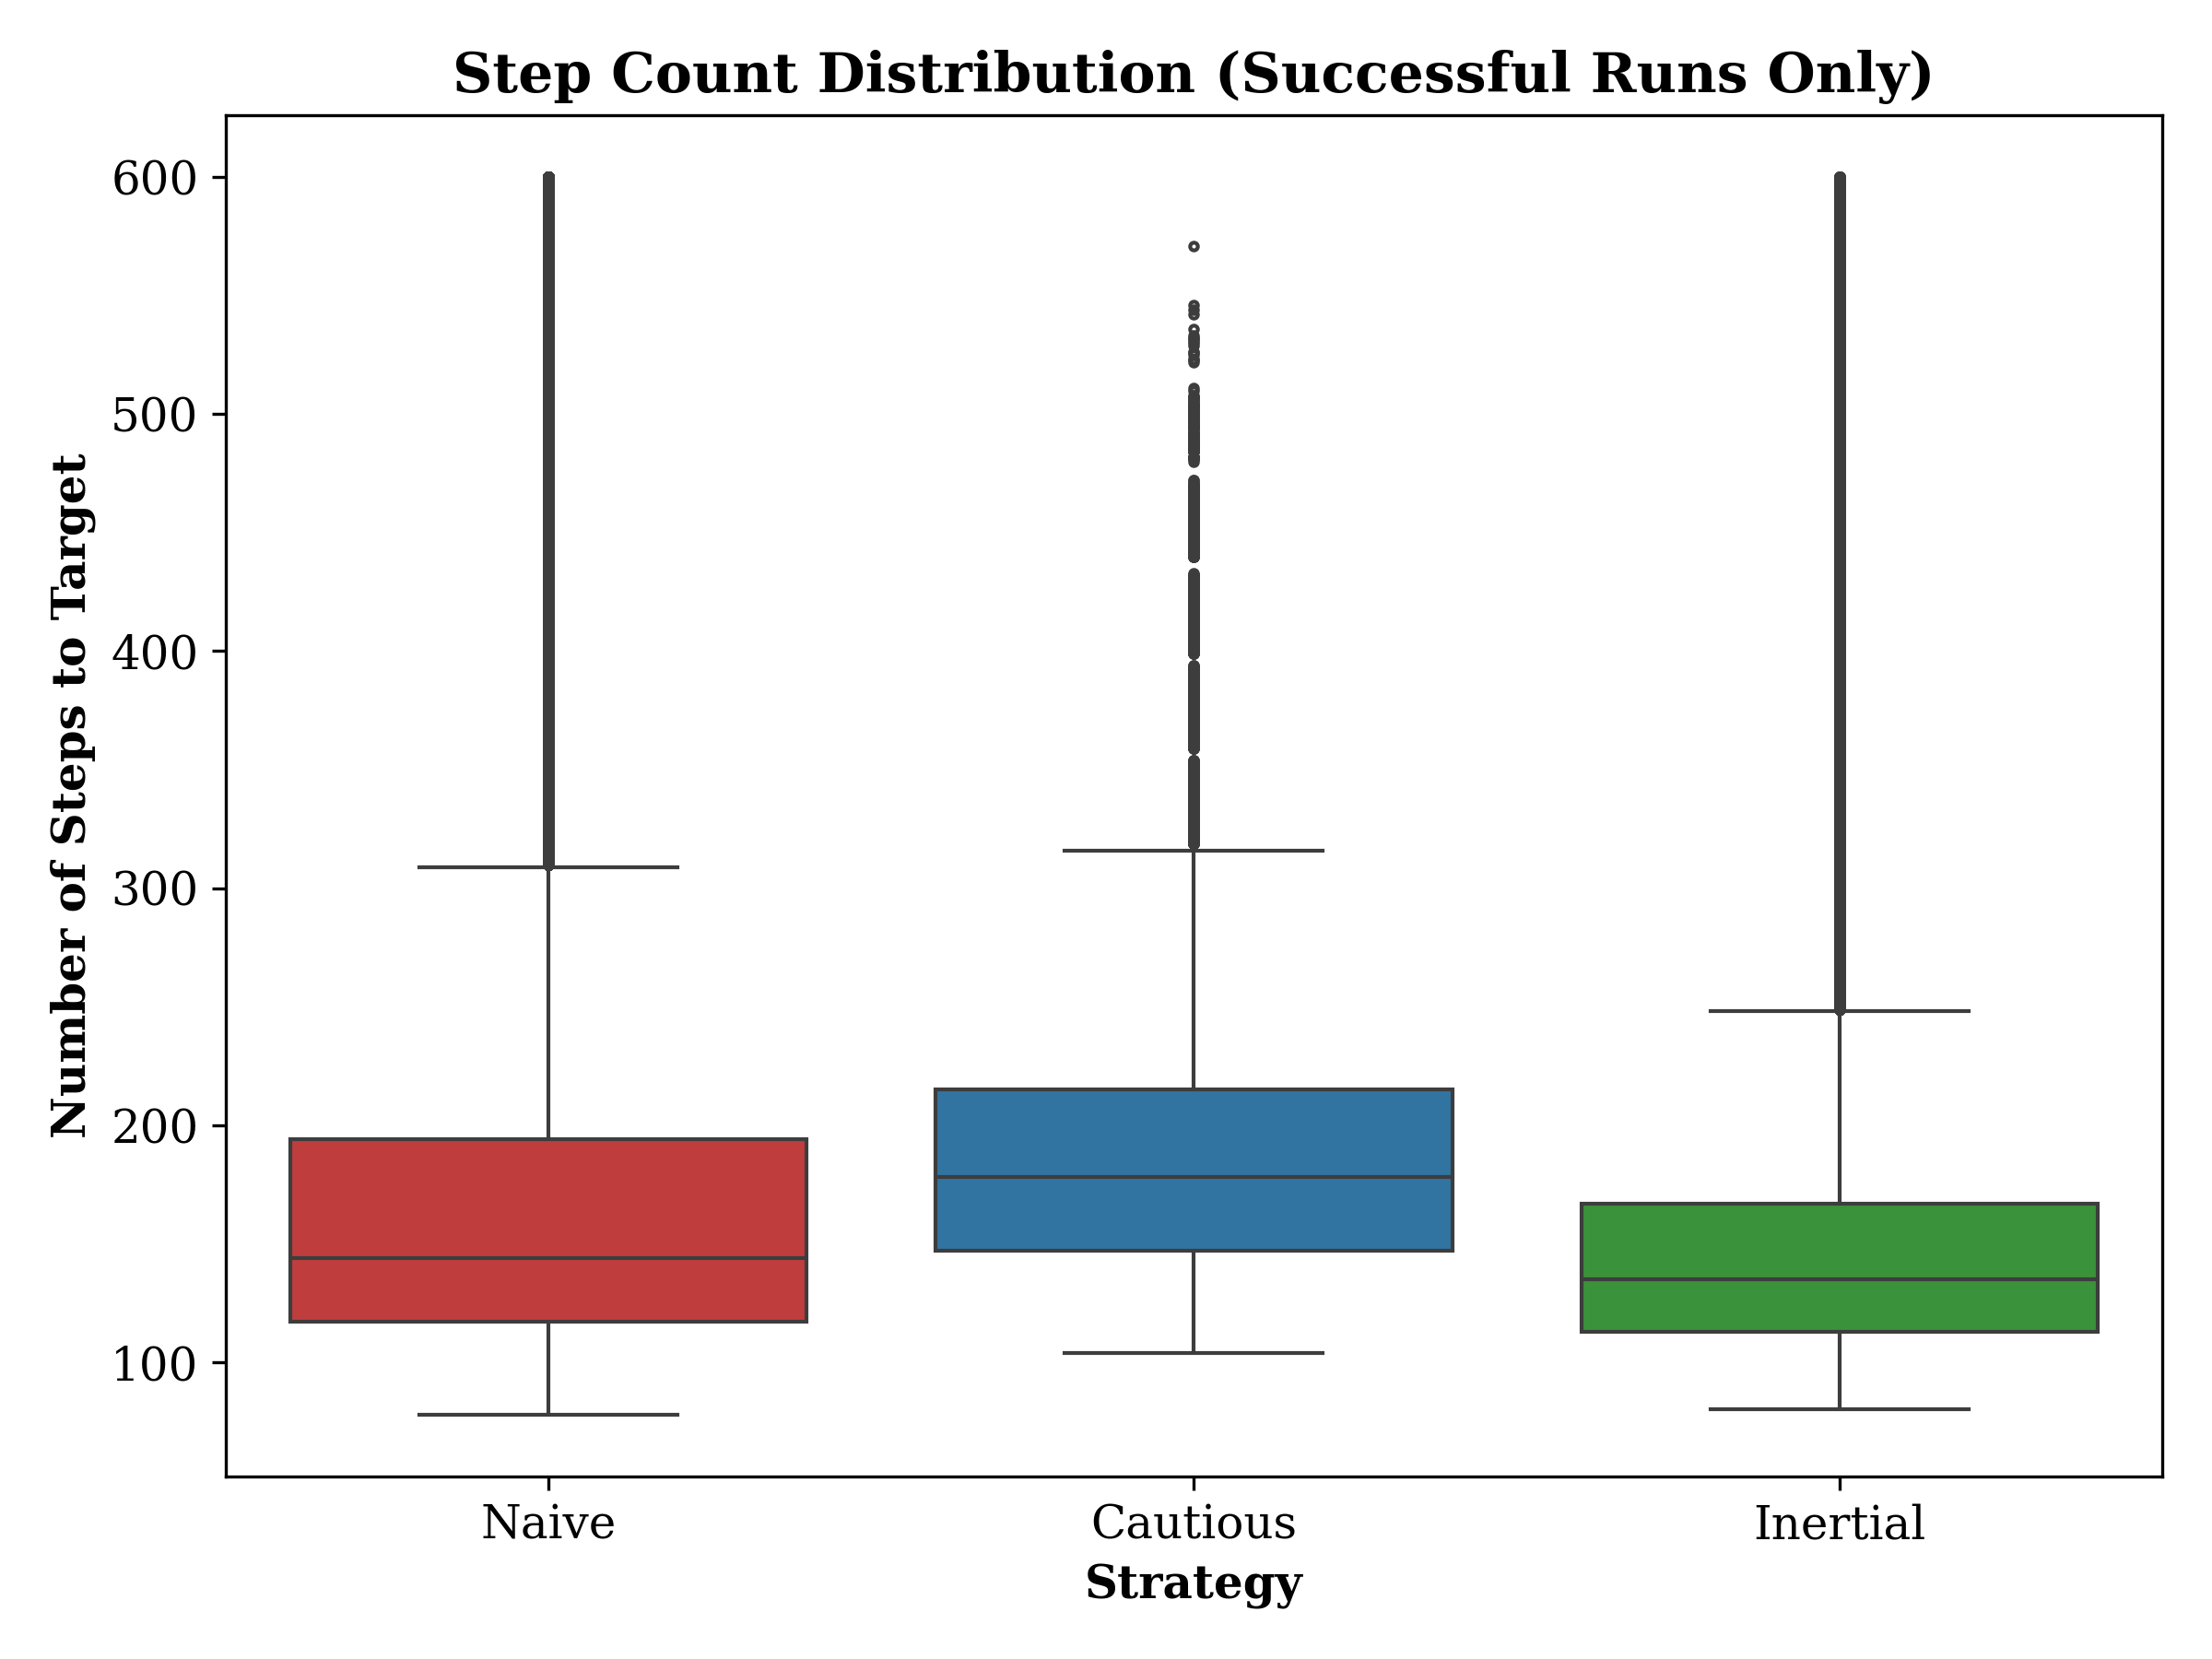
\includegraphics[width=0.9\linewidth]{steps_distribution.png}
    \caption{Distribution of step counts required to reach the target for successful runs. The Cautious strategy exhibits a higher median cost due to adversarial pausing, whereas the Inertial heuristic optimizes speed at the cost of theoretical safety.}
    \label{fig:steps_dist}
\end{figure}

While the Cautious strategy provides absolute theoretical safety, Table \ref{tab:efficiency} and Fig. \ref{fig:steps_dist} reveal a significant operational trade-off. By freezing its spatial movement during every detected adversarial burst, the Cautious robot incurs a distinct temporal penalty, requiring an average of 189 steps to complete the navigation. 

Conversely, the Inertial heuristic optimizes for time by continuing its geometric traversal during spoofed periods, reducing the average path duration to approximately 148 steps—a 21.7\% efficiency improvement over the Cautious approach. This establishes a fundamental design paradigm for autonomous agents under adversarial conditions: one must explicitly choose between absolute convergence guarantees (Cautious) and average-case temporal efficiency (Inertial).

\begin{figure}[htbp]
    \centering
    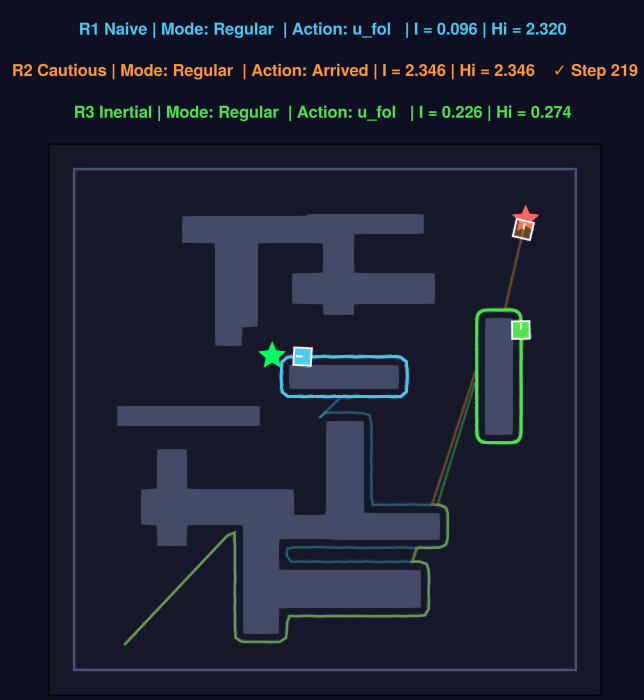
\includegraphics[width=0.8\linewidth]{simulation_trap.png}
    \caption{A visualization of the Cyclic Synchronization trap. The Inertial robot (green) is caught in an infinite boundary-following loop due to open-loop navigation during spoofing, while the Cautious robot (orange) successfully breaks the cycle by pausing.}
    \label{fig:sim_trap}
\end{figure}

\section{Limitations and Future Work}
While the Cautious strategy provides strong theoretical guarantees against intermittent additive spoofing, the current mathematical framework relies on specific assumptions that define clear avenues for future research:

\begin{itemize}
    \item \textbf{Sensor Noise and Stochastic Filtering:} The current anomaly detection mechanism relies on identifying a near-instantaneous mathematical discontinuity ($\frac{\partial S}{\partial t} \to \infty$). In physical hardware deployments, high Gaussian noise, multipath fading, or environmental attenuation could trigger false positives or obscure true anomalies. Future iterations must incorporate probabilistic estimators (e.g., Extended Kalman Filters or Particle Filters) to smooth sensor readings and dynamically adapt anomaly thresholds.
    
    \item \textbf{Gradient-Ramping Attacks:} The security of the algorithm assumes the adversarial transmitter activates as a discrete step function. If an intelligent adversary continuously and gradually ramps up its signal strength to perfectly mimic the robot's maximum physical spatial derivative ($K \cdot v_{max}$), the temporal anomaly filter would fail to trigger. This ``gradient hijacking" would allow the superimposed signal to misdirect the robot undetected, presenting a significant theoretical vulnerability.
    
    \item \textbf{Resonance Breaking in Heuristics:} The empirical discovery of Cyclic Synchronization trapping in the Inertial strategy highlights a fundamental topological vulnerability in open-loop heuristics. Future work could explore stochastic resonance-breaking mechanisms—such as randomizing the robot's physical step size or introducing angular jitter during blind boundary following—to probabilistically escape these mathematical traps without incurring the full temporal penalty of the Cautious strategy.
    
    \item \textbf{Dynamic Mobile Adversaries:} The mathematical proof provided in Theorem 1 relies on a stationary adversarial source. The spatial dynamics of a mobile adversary actively pursuing the robot or continuously altering its transmission location introduce shifting false gradients that require a fundamentally different theoretical approach to state preservation.

\item \textbf{Physical Implementation and Hardware Testing:} The original I-Bug framework was successfully validated on a physical differential-drive robot (Lego Mindstorms with IR sensors) \cite{taylor2014intensity}. Future work must transition our proposed robust strategies from kinematic simulations to physical hardware. Evaluating the anomaly-detection filter under real-world conditions—such as hardware latency, sensor discretization, and physical multipath fading—will be critical to fully realizing adversarially robust minimalist robotics.
\end{itemize}

\section{Conclusion}
This paper addressed a critical theoretical vulnerability in minimalist, intensity-based navigation frameworks such as the I-Bug algorithm: catastrophic susceptibility to adversarial signal spoofing governed by physical wave superposition. We demonstrated that a computationally constrained autonomous agent can successfully reject additive adversarial interference by extracting temporal cues from spatial signal data, leveraging the strict physical bounds of its own kinematics. 

Through the introduction of the anomaly-detecting Cautious strategy, we mathematically proved that absolute target convergence and strict geometric path bounds can be preserved by entirely suspending spatial movement and state updates during spoofed periods. Our massive-scale simulation across 1,000,000 procedurally generated environments empirically validated these claims, yielding a 100\% success rate for the Cautious approach. 

Furthermore, our comparative analysis highlighted a fundamental operational trade-off in adversarial robotics. While the standard Naive baseline failed in 42.57\% of cases, the proposed Inertial heuristic optimized average execution time by 21.7\% relative to the Cautious strategy. However, this temporal efficiency came at the cost of absolute safety, leaving the Inertial robot vulnerable to highly specific topological traps (Cyclic Synchronization) resulting in a 99.11\% success rate. Ultimately, this work establishes a mathematically rigorous foundation for developing secure, sensor-minimalist autonomous navigation systems capable of operating reliably in contested and deceptive environments.

\bibliographystyle{plain}
\begin{thebibliography}{9}

\bibitem{lumelsky1987path}
V. J. Lumelsky and A. A. Stepanov, ``Path-planning strategies for a point mobile automaton moving amidst unknown obstacles of arbitrary shape,'' \textit{Algorithmica}, vol. 2, no. 1, pp. 403--430, 1987.

\bibitem{kamon1998tangentbug}
I. Kamon, E. Rivlin, and E. Rimon, ``A new range-sensor based universally convergent obstacle avoidance algorithm,'' \textit{IEEE Trans. Robot. Autom.}, vol. 14, no. 2, pp. 227--233, Apr. 1998.

\bibitem{taylor2009ibug}
K. Taylor and S. M. LaValle, ``I-Bug: An intensity-based bug algorithm,'' in \textit{Proc. IEEE Int. Conf. Robot. Autom. (ICRA)}, Kobe, Japan, 2009, pp. 3981--3986.

\bibitem{taylor2014intensity}
K. Taylor and S. M. LaValle, ``Intensity-based navigation with global guarantees,'' \textit{Autonomous Robots}, vol. 36, no. 4, pp. 349--364, 2014.

\end{thebibliography}

\end{document}